\section{Propuesta}

En esta sección detallaremos el objetivo de la propuesta y los detalles técnicos para el desarrollo de la misma.

\subsection{Plataforma implementada}

En este trabajo se propone el desarrollo de una plataforma para el análisis de secuencias scRNA.  Por ejemplo en la Figura \ref{fig:analysis}, se presente las fases tradicionales de una análisis de secuencias de ADN (Next-generation). En este caso, vemos como se realiza el secuenciamiento de ADN/ARN, obteniendo miles y millones de lecturas cortas de la cadena de ADN. Entonces la idea es analizar estas secuencias con el fin de  saber que genes estan activos y como influye esto en el fenotipo de la especie. Por ejemplo, este análisis se suele realizar sobre celulas de tejido tumoral y se compara con otro experimiento que tomo muestras de celulas sanas, luego de una comparación se puede determinar cuales son los genes activos o inactivos según el tipo de tumor y enfermedad, esto nos ayuda a comprender mejor las enfermedades y mas aún detectarlas en fases tempranas. \\

Como se menciono antes, la propuesta se base en el desarrollo de una plataforma que permita un análisis de secuencias de ADN sobre un sistema distribuido. Realizar todo el análisis es costoso, debido a eso \textbf{en esta etapa se desarrollo en la verificación de calidad de las secuencias} de entrada. En proyectos futuros se completará la plataforma con mas funcionalidades. \\

\begin{figure}[H]
    \centering
    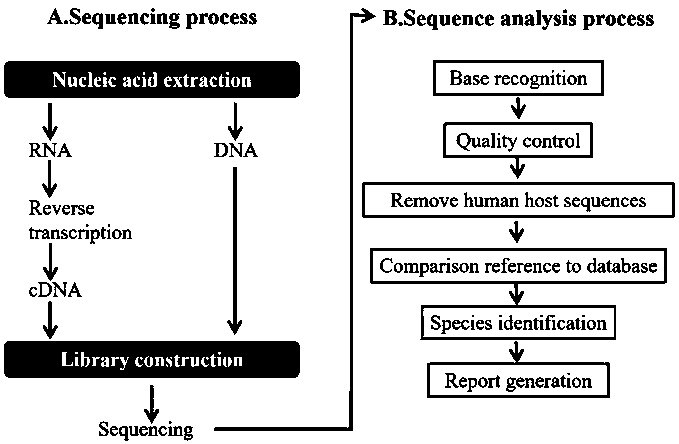
\includegraphics[width=0.6\textwidth]{img/proy/analysis2}
    \caption{Phases comunes realizadas en un análisis de secuencias de ADN (Next-generation).}
    \label{fig:analysis}
\end{figure}

\subsection{Herramientas utilizadas}

Para el desarrollo de la propuesta se ha utilizado las herramientas de la Tabla \ref{tab:tools}. Se escogio, Spark, debido a su versatilidad y la gestión de RDDs que permiten un desarrollo distribuido facil de implementar. Luego, se opto por utilizar Pyspark, porque la evaluación de los \textit{scripts} pueden hacerse desde el interprete de Python y incluso en Google Colab, esto es una ventaja porque reduce el tiempo de desarrollo.\\

\begin{table}[H]
	\centering
	\caption{Herramientas utilizadas para el proyecto}
	\label{tab:tools}
	\begin{tabular}{ll}
		\textbf{Herramienta} & \textbf{Version}
		\\ \hline
		Spark       & 3.2.0   \\
		Python      & 3.8.10  \\
		Pyspark     & 3.2.0  
	\end{tabular}
\end{table}

\subsection{Hardware}

En cuanto al hardware utilizado en el sistema distribuido, este es detallado en la Tabla \ref{tab:pcs}. Debido a la falta de recursos, solo se utilizo dos computadoras, una es un minicomputador Asus y una laptop Asus Taichi (ver Figura \ref{img:pcs})\\


\begin{table}[H]
	\centering
	\caption{Computadoras utilizadas en el sistema distribuído}
	\label{tab:pcs}
	\begin{tabular}{lp{8cm}}
		\textbf{Nombre de PC} & \textbf{Especificaciones}
		\\ \hline
		Desktop Asus      & Procesador i7 de séptima generación y 8GB de memoria RAM. Sistema operativo Linux.   \\
		Laptop Asus      & Procesador i5 de quinta generación y 4GB de memoria RAM. Sistema operativo Linux.\\
	\end{tabular}
\end{table}


 \begin{figure}[H]
	\centering
	\begin{multicols}{2}
		
\includegraphics[width=\textwidth,height=0.2\textheight,keepaspectratio]{img/proy/pc_asus_1}\par 
		
\includegraphics[width=\textwidth,height=0.2\textheight,keepaspectratio]{img/proy/pc_asus_2}\par 
	\end{multicols}
	\caption{Computadoras utilizadas en el sistema distribuído.}
	\label{img:pcs}
\end{figure}

\subsection{Funcionalidades}

Las funcionalidades de la propuesta son:
\begin{itemize}
	\item Conteo de la cantidad de secuencias. 
	\item Conteo total de las bases nitrogenadas. 
	\item Computo de la longitud de todas las secuencias. 
	\item Computo del promedio de las longitudes de las secuenias.
	\item Computo de la ocurrencia de cada base nitrogenada.
	\item Análisis de contenido por base.
\end{itemize}

\subsection{Implementación}

El código fuente de la propuesta está en \href{La implementación esta en un  repositorio de Github }{esté repositorio}. Lineas abajo, presentamos un extracto del archivo principal. \\

\begin{lstlisting}
# este codigo, realiza un pequenio analisis a vcarias secuencias scRNA, 
# se considero a ERR3014700. Se usa SRA toolkit para genera el archivo fasta.

from __future__ import print_function
from functools import wraps
import pyspark as spark
from pyspark import SparkConf
import time
from operator import add
import os 
from subprocess import STDOUT, check_call, check_output


class Fastq:
	def __init__(self, path:str) -> str:
		self.path = path
		self.stop_context()
		self.sc = spark.SparkContext.getOrCreate(conf=self.set_conf())
		self.data = self.sc.textFile(self.path)
	
	def stop_context(self):
		try:
			self.sc.stop()
			except:
		pass
	
	def set_conf(self):
		conf = SparkConf().setAppName("App")
		conf = (conf.setMaster('local[*]')
		.set('spark.executor.memory', '4G')
		.set('spark.driver.memory', '16G')
		.set('spark.driver.maxResultSize', '8G'))
		return conf

	def _logging(func):
	@wraps(func)
	def log_print(instance, *args, **kwargs):
		start = time.time()
		res = func(instance, *args, **kwargs)
		print("Finished Executing {}  in {}s!".format(func.__name__, time.time() - start))
		return res
		return log_print

	@_logging
	def get_data(self):
	return self.data

	@_logging
	def count_bases(self):
		seqs = self.extract_seq()
		seqs = seqs.flatMap(lambda line: list(line)) 
		seqs = seqs.map(lambda c: (c, 1))
		return seqs.reduceByKey(lambda a, b: a+b)#\
	
	
	@_logging
	def per_base_seq_content(self):
		seqs = self.extract_seq()
		seqs = seqs.flatMap(lambda line: list(line)) 
		seqs = seqs.map(lambda c: (c, 1))
		return seqs.reduceByKey(lambda a, b: a+b)#\
	
	@_logging
	def extract_seq(self):
		return self.data.filter(lambda x: x.isalpha())
	
	@_logging
	def get_lengths(self):
		seqs = self.extract_seq()
		return seqs.map(lambda x: len(x))
	
	def extract_qual(self):
		pass
	
	def extract_meta(self):
		pass


fasta = Fastq('/home/vicente/Documents/sratoolkit.2.11.3-ubuntu64/samples/ERR3014700.fastq')

# show first read
print("fasta head:", fasta.data.take(4))

# show read count
print("Read count:", fasta.data.count())

# extract sequences alone from the fastq file
seqs = fasta.extract_seq()

print("total sequences:", seqs.count())
print("sequences:", seqs.take(4))

# compute read lengths
lens = fasta.get_lengths()

# show the lengths of the first 10 reads
print("sequence lenghts:", lens.take(10))

# get the average read length
len_sum = lens.reduce(lambda x, y: x+y)
print("sequence mean lenght:", len_sum//lens.count())

# count base occurance
bases = fasta.count_bases()
print("Bases ocurrence:", bases.take(10))

import json
file = open("results.txt", "w")
results = {
'bases':  fasta.data.count(),
'total_seqs': seqs.count(),  
'seqs_len': lens.take(10),
'seqs_len_mean': len_sum//lens.count(),
'bases_ocurrence': bases.take(10)
}
file.write( json.dumps(results, indent=4) )

######################################################
# procesamos per base sequence content
#######################################################
seqs = fasta.extract_seq()

# get max, min, mean lenght
lens = fasta.get_lengths()
len_max = lens.reduce(lambda x, y: max(x, y))
len_min = lens.reduce(lambda x, y: min(x, y))
len_sum = lens.reduce(lambda x, y: x+y)
len_mean = len_sum//lens.count()

print(len_max, len_min, len_mean)

import numpy as np

# vectores de las 4 bases, para el conteo
#list_a = fasta.sc.parallelize(np.zeros( len_max ))
#list_c = fasta.sc.parallelize(np.zeros( len_max ))
#list_g = fasta.sc.parallelize(np.zeros( len_max ))
#ist_t = fasta.sc.parallelize(np.zeros( len_max ))

list_a = np.zeros( len_max )
list_c = np.zeros( len_max )
list_g = np.zeros( len_max )
list_t = np.zeros( len_max )

lens = fasta.get_lengths()
lens_np = np.array(lens.collect())

#for i in range( 3 ): # por cada base 
for i in range( len_max ):
if i < lens_np[i]:
acc_a = seqs.map(lambda x: x[i] if i < len(x)  else 'X' ).filter( lambda x: x=='A').count()
acc_c = seqs.map(lambda x: x[i] if i < len(x)  else 'X' ).filter( lambda x: x=='C').count()
acc_g = seqs.map(lambda x: x[i] if i < len(x)  else 'X' ).filter( lambda x: x=='G').count()
acc_t = seqs.map(lambda x: x[i] if i < len(x)  else 'X' ).filter( lambda x: x=='T').count()

list_a[i] = acc_a
list_c[i] = acc_c
list_g[i] = acc_g
list_t[i] = acc_t


n_seqs = seqs.count()
list_a = list_a/n_seqs
list_c = list_c/n_seqs
list_g = list_g/n_seqs
list_t = list_t/n_seqs

import matplotlib.pyplot as plt

plt.plot(range(len_max), list_a)
plt.plot(range(len_max), list_c)
plt.plot(range(len_max), list_g)
plt.plot(range(len_max), list_t)
#plt.show()
plt.savefig('per_base_content.png', bbox_inches='tight')
\end{lstlisting}


